% AC5211 Multimedia Database -- final report.
% Build:  python3 scripts/gen_results.py && latexmk -pdf main.tex
% Every number from our own runs comes from generated/numbers.tex (results/*.csv);
% numbers quoted from IRRA are typed inline next to a citation.
\documentclass[conference,a4paper]{IEEEtran}

\usepackage[utf8]{inputenc}
\usepackage[T1]{fontenc}
\usepackage{cite}
\usepackage{amsmath,amssymb,amsfonts}
\usepackage{graphicx}
\usepackage{textcomp}
\usepackage{xcolor}
\usepackage{array}
\usepackage{booktabs}
\usepackage{multirow}
\usepackage{tabularx}
\usepackage{tikz}
\usetikzlibrary{positioning,arrows.meta,fit,calc,backgrounds}
\usepackage{pgfplots}
\pgfplotsset{compat=1.18}
\usepackage[hidelinks]{hyperref}
\usepackage[capitalize,nameinlink]{cleveref}

% AUTO-GENERATED by scripts/gen_results.py -- do not edit by hand.
\newcommand{\sdmPeakEp}{9}
\newcommand{\sdmPeakR}{58.85}
\newcommand{\sdmPeakRfive}{80.30}
\newcommand{\sdmPeakRten}{89.15}
\newcommand{\sdmPeakM}{45.46}
\newcommand{\sdmPeakMINP}{23.29}
\newcommand{\sdmBestM}{45.56}
\newcommand{\sdmBestMEp}{14}
\newcommand{\sdmConvR}{57.18}
\newcommand{\sdmConvRsd}{0.28}
\newcommand{\sdmConvM}{45.42}
\newcommand{\sdmConvMsd}{0.13}
\newcommand{\sdmEpochs}{20}
\newcommand{\sdmLastR}{56.95}
\newcommand{\sdmDrop}{1.90}
\newcommand{\sdmLossFirst}{21.16}
\newcommand{\sdmLossLast}{8.07}
\newcommand{\sdmEpNineR}{58.85}
\newcommand{\sdmEpFourR}{55.50}
\newcommand{\sdmEpThreeR}{52.55}
\newcommand{\sdmMinPerEp}{7.2}
\newcommand{\mpcePeakEp}{3}
\newcommand{\mpcePeakR}{55.70}
\newcommand{\mpcePeakRfive}{76.40}
\newcommand{\mpcePeakRten}{85.50}
\newcommand{\mpcePeakM}{42.35}
\newcommand{\mpcePeakMINP}{20.78}
\newcommand{\mpceBestM}{42.92}
\newcommand{\mpceBestMEp}{5}
\newcommand{\mpceConvR}{48.85}
\newcommand{\mpceConvRsd}{0.15}
\newcommand{\mpceConvM}{40.82}
\newcommand{\mpceConvMsd}{0.06}
\newcommand{\mpceEpochs}{30}
\newcommand{\mpceLastR}{49.00}
\newcommand{\mpceDrop}{6.70}
\newcommand{\mpceLossFirst}{4.26}
\newcommand{\mpceLossLast}{0.61}
\newcommand{\mpceEpNineR}{51.05}
\newcommand{\mpceEpFourR}{53.65}
\newcommand{\mpceEpThreeR}{55.70}
\newcommand{\mpceMinPerEp}{6.9}
\newcommand{\ncePeakEp}{3}
\newcommand{\ncePeakR}{55.20}
\newcommand{\ncePeakRfive}{76.65}
\newcommand{\ncePeakRten}{85.25}
\newcommand{\ncePeakM}{42.15}
\newcommand{\ncePeakMINP}{20.64}
\newcommand{\nceBestM}{43.07}
\newcommand{\nceBestMEp}{6}
\newcommand{\nceConvR}{48.52}
\newcommand{\nceConvRsd}{0.25}
\newcommand{\nceConvM}{40.56}
\newcommand{\nceConvMsd}{0.14}
\newcommand{\nceEpochs}{27}
\newcommand{\nceLastR}{48.60}
\newcommand{\nceDrop}{6.60}
\newcommand{\nceLossFirst}{2.10}
\newcommand{\nceLossLast}{0.29}
\newcommand{\nceEpNineR}{51.75}
\newcommand{\nceEpFourR}{53.80}
\newcommand{\nceEpThreeR}{55.20}
\newcommand{\nceMinPerEp}{6.6}
\newcommand{\gapSdmNceR}{3.65}
\newcommand{\gapSdmNceM}{3.31}
\newcommand{\gapSdmMpceR}{3.15}
\newcommand{\gapSdmMpceM}{3.11}
\newcommand{\gapSdmMpceBestM}{2.64}
\newcommand{\mpNceDiffR}{0.18}
\newcommand{\mpNceDiffRsd}{0.59}
\newcommand{\mpNceDiffRmax}{1.45}
\newcommand{\mpNceDiffM}{0.17}
\newcommand{\mpNceDiffMmax}{0.64}
\newcommand{\lossRatioLo}{2.03}
\newcommand{\lossRatioHi}{2.12}
\newcommand{\nPairedEp}{27}
\newcommand{\sdmLrFour}{9.92}
\newcommand{\sdmLrNine}{7.26}
\newcommand{\nceLrFour}{9.97}
\newcommand{\nceLrNine}{8.84}
\newcommand{\lrMaxRelDiff}{18}
\newcommand{\gapIrraR}{1.35}
\newcommand{\gapIrraM}{1.71}
\newcommand{\gapIrraSdmR}{1.65}
\newcommand{\gainIrraSdm}{3.15}
\newcommand{\nTrainable}{491\,520}
\newcommand{\nTotal}{150\,109\,185}
\newcommand{\nTotalM}{150.1}
\newcommand{\nBackbone}{149\,617\,665}
\newcommand{\nBackboneM}{149.6}
\newcommand{\trainPct}{0.33}
\newcommand{\nLoraModules}{96}
\newcommand{\ckptMiB}{1.88}
\newcommand{\fullMiB}{571}
\newcommand{\sizeRatio}{304}
\newcommand{\idHeadM}{1.90}
\newcommand{\batchSize}{64}
\newcommand{\sdmRounds}{20}
\newcommand{\nceRounds}{30}
\newcommand{\mpceRounds}{30}
\newcommand{\posFrac}{1.52}
\newcommand{\oneHotFrac}{98.48}
\newcommand{\nExamples}{37\,010}
\newcommand{\logInvEps}{18.42}
\newcommand{\kClients}{15}
\newcommand{\rRounds}{30}
\newcommand{\upLoraRoundMiB}{28.1}
\newcommand{\upFullRoundGiB}{8.4}
\newcommand{\upLoraTotalGiB}{0.82}
\newcommand{\upFullTotalGiB}{251}
\newcommand{\optLoraMiB}{3.75}
\newcommand{\optFullGiB}{1.11}
\newcommand{\roundVsOneFull}{20}


% series colours (validated categorical palette; also distinguished by marker/dash)
\definecolor{cSDM}{HTML}{2A78D6}
\definecolor{cMPCE}{HTML}{EB6834}
\definecolor{cNCE}{HTML}{1BAF7A}
\definecolor{cOurs}{HTML}{2A78D6}
\definecolor{cIRRA}{HTML}{6B6B6B}

\newcommand{\ours}[1]{\textcolor{cOurs}{#1}}
\newcommand{\tagE}{\textsc{[Existing]}}
\newcommand{\tagO}{\textsc{[Ours]}}
\DeclareMathOperator{\KL}{KL}

\begin{document}

\title{LoRA Meets Similarity Distribution Matching:\\
Parameter-Efficient CLIP Tuning for Text-Based Person Search}

\author{\IEEEauthorblockN{\DJ{}\~{\^o} Thanh T\`ung}
\IEEEauthorblockA{Student ID: 20252432M\\
AC5211 Multimedia Database --- Final Report\\
Hanoi, Vietnam}}

\maketitle

\begin{abstract}
Text-based person search retrieves images of a pedestrian from a large gallery given a free-form description. This report is drawn from an ongoing master's thesis on parameter-efficient fine-tuning (PEFT) for federated text-based person search. In federated learning every client uploads its update in every round, so the size of the trainable part sets the communication cost, and a premise must hold before federating: a far smaller update must lose little accuracy. We test this premise centrally on IRRA, the method of our midterm presentation, which fine-tunes all of CLIP with the Similarity Distribution Matching (SDM) loss. Freezing CLIP and attaching rank-4 LoRA to the attention projections of both encoders, we train \nTrainable{} parameters instead of \nBackboneM\,M, \sizeRatio$\times$ fewer (a \ckptMiB\,MiB instead of a \fullMiB\,MiB update). With SDM as the sole objective the model reaches \sdmPeakR\% Rank-1 on RSTPReid at its best epoch and \sdmConvR\% once converged, on par with the 57.20\% IRRA reports for full fine-tuning with SDM alone; in a \kClients-client federation the per-round upload would fall from \upFullRoundGiB\,GiB to \upLoraRoundMiB\,MiB. We also ask where SDM's gain over the standard contrastive loss comes from. Under the random batch sampling IRRA uses, only \posFrac\% of batch rows contain a second positive, so SDM's target is almost always one-hot; there SDM does \emph{not} reduce to InfoNCE but to a scaled mean-absolute-error term plus an entropy bonus. A control loss with SDM's targets and the opposite KL direction tracks InfoNCE to within \mpNceDiffR{} Rank-1 points on average and trails SDM by \gapSdmMpceR{} points, attributing the gain to the divergence direction rather than to multi-positive supervision.
\end{abstract}

\begin{IEEEkeywords}
text-based person search, cross-modal retrieval, CLIP, LoRA, parameter-efficient fine-tuning, federated learning, contrastive loss
\end{IEEEkeywords}

\section{Introduction}\label{sec:intro}

Text-based person search (TBPS) ranks a gallery of pedestrian images against a natural-language query such as ``a woman in a white coat carrying a black backpack''~\cite{li2017personsearchnaturallanguage}. It is a cross-modal retrieval problem of the kind multimedia databases are built to serve: the gallery is indexed once by an image encoder, each query is embedded by a text encoder, and retrieval reduces to a nearest-neighbour search in a shared embedding space. Its difficulty lies in granularity: every gallery item is a person, so the description must separate individuals who differ only in a garment's colour or a carried object.

Vision--language models pre-trained on web-scale image--text pairs, CLIP in particular~\cite{radford2021learningtransferablevisualmodels}, now provide the backbone of the strongest TBPS methods~\cite{yan2022clipdrivenfinegrainedtextimageperson,cao2023empiricalstudycliptextbased}. IRRA~\cite{jiang2023crossmodalimplicitrelationreasoning}, the CVPR~2023 paper we presented at midterm, fine-tunes the entire CLIP ViT-B/16 backbone together with three objectives: an implicit relation reasoning (IRR) branch, an identity (ID) classification loss, and the Similarity Distribution Matching (SDM) loss. Two aspects of this recipe motivate the present work. Full fine-tuning updates and stores every one of the backbone's \nBackboneM\,M parameters, and IRRA's own ablation shows that SDM is the single component that contributes most on RSTPReid~\cite{Zhu_2021}. Parameter-efficient transfer learning (PETL) methods for TBPS~\cite{liu2024clipbasedsynergisticknowledgetransfer,liu2025dmadapterdomainawaremixtureofadapterstextbased,liu2025uppersonunifiedparameterefficienttransfer} have since shown that a frozen backbone can compete, but they still train millions of parameters and combine several modules, so the contribution of the loss is hard to isolate.

\textbf{Context and goal.} The experiments in this report are drawn from the author's master's thesis, which studies PEFT of foundation models in federated learning (FL), with TBPS as the application. Surveillance images belong to operators that often cannot pool them, so the model has to be trained where the data reside~\cite{mcmahan2023communicationefficientlearningdeepnetworks,Ma_2024}. FL pays for the trainable part repeatedly: every client receives and returns it in every round, for tens of rounds, often over limited links~\cite{Ma_2024}. With full fine-tuning of CLIP that is \fullMiB\,MiB per client per round. Before the federated difficulties (non-IID clients, aggregation) are even reached, one premise must hold: \emph{a much smaller trainable part must lose little accuracy}. This course report establishes that premise in the centralised setting, where it can be measured cleanly; the federated experiments belong to the thesis and are outside its scope.

We therefore study the most reduced configuration we could construct: a frozen CLIP backbone, low-rank adaptation (LoRA)~\cite{hu2021loralowrankadaptationlarge} of the attention projections, and SDM as the only objective. Two questions guide the report. \textbf{(Q1)} How much accuracy does this configuration give up relative to IRRA's fully fine-tuned counterpart, and how much does it save? \textbf{(Q2)} Why does SDM outperform the InfoNCE loss~\cite{oord2019representationlearningcontrastivepredictive} used by CLIP? Q2 serves the same goal: SDM is the only IRRA objective with no parameters tied to the global identity set, hence the one that carries over to FL unchanged, and whether its gain persists on clients holding few images per person depends on why it helps. IRRA attributes the gain to SDM's ability to treat all same-identity pairs in a batch as positives; we test this explanation directly.

\textbf{Contributions.} Because this is a course report building on a paper we studied, \cref{tab:contrib} states which parts are taken from prior work and which are ours, and the section headings carry the tags \tagE{} and \tagO{}. Our contributions are:
\begin{enumerate}
  \item A LoRA+SDM pipeline for TBPS that trains \trainPct\% of CLIP's parameters and reaches \sdmPeakR\% (peak) / \sdmConvR\% (converged) Rank-1 on RSTPReid, against 57.20\% for IRRA's full fine-tuning with SDM alone (\cref{sec:main}), with an accounting of what this saves in storage, optimiser memory and federated communication (\cref{sec:fl}).
  \item An analysis of SDM under identity labels: a closed-form decomposition showing that it does not reduce to InfoNCE when each identity appears once in a batch, its gradient, and the observation that this one-hot regime covers \oneHotFrac\% of batch rows under random sampling (\cref{sec:analysis}).
  \item A controlled loss ablation under LoRA, including a multi-positive cross-entropy (MPCE) control that we designed to separate the effect of identity-aware targets from that of the KL direction (\cref{sec:ablation}).
\end{enumerate}

\begin{table}[t]
\centering
\caption{What this report takes from prior work and what it adds.}
\label{tab:contrib}
\footnotesize
\setlength{\tabcolsep}{3pt}
\begin{tabularx}{\columnwidth}{@{}>{\raggedright\arraybackslash}p{0.43\columnwidth}>{\raggedright\arraybackslash}X@{}}
\toprule
\textbf{Existing (source)} & \textbf{Ours} \\
\midrule
CLIP ViT-B/16 dual encoder~\cite{radford2021learningtransferablevisualmodels}; $384{\times}128$ input with interpolated position embeddings, $\tau{=}0.02$ (IRRA) & Choice of a frozen backbone with LoRA on Q/K/V/O of \emph{both} encoders; rank, scaling, schedule; implementation and training code \\
\addlinespace
SDM loss, InfoNCE baseline and ablation numbers on RSTPReid (IRRA~\cite{jiang2023crossmodalimplicitrelationreasoning}) & SDM as the \emph{sole} objective; all LoRA results; parameter, storage and communication accounting \\
\addlinespace
LoRA~\cite{hu2021loralowrankadaptationlarge}; MAE robustness~\cite{ghosh2017robustlossfunctionslabel}; confidence penalty~\cite{pereyra2017regularizingneuralnetworkspenalizing} & Decomposition and gradient of SDM with one-hot targets; in-batch positive rate; link to MAE and entropy bonus \\
\addlinespace
RSTPReid and its protocol~\cite{Zhu_2021} & MPCE control loss; InfoNCE/MPCE/SDM ablation; attribution of SDM's gain to the KL direction \\
\bottomrule
\end{tabularx}
\end{table}

\section{Related Work}\label{sec:related}

\textbf{Text-based person search.} Li~\textit{et al.}~\cite{li2017personsearchnaturallanguage} introduced the task with CUHK-PEDES; ICFG-PEDES~\cite{ding2021semanticallyselfalignednetworktexttoimage} and RSTPReid~\cite{Zhu_2021}, both built from MSMT17 imagery, followed. Early methods paired separately pre-trained image and text networks and aligned them with identity-aware objectives, most notably the cross-modal projection matching and classification losses CMPM/CMPC~\cite{Zhang_2018}, often complemented by explicit part- or phrase-level alignment~\cite{ding2021semanticallyselfalignednetworktexttoimage}. CLIP changed the starting point: CFine~\cite{yan2022clipdrivenfinegrainedtextimageperson} and the empirical study of Cao~\textit{et al.}~\cite{cao2023empiricalstudycliptextbased} show that a jointly pre-trained image--text model outperforms these specialised designs, and IRRA~\cite{jiang2023crossmodalimplicitrelationreasoning} combines full CLIP fine-tuning with masked-language-model-based relation reasoning and the SDM loss. Our work keeps IRRA's backbone and loss but removes everything else.

\textbf{Parameter-efficient transfer.} PETL freezes a pre-trained model and trains a small inserted component: bottleneck adapters~\cite{houlsby2019parameterefficienttransferlearningnlp}, learned prefixes~\cite{li2021prefixtuningoptimizingcontinuousprompts}, or LoRA~\cite{hu2021loralowrankadaptationlarge}, which adds a trainable low-rank update to frozen weight matrices and can be merged into them after training. For TBPS, CSKT~\cite{liu2024clipbasedsynergisticknowledgetransfer} transfers CLIP knowledge with prompts and adapters, DM-Adapter~\cite{liu2025dmadapterdomainawaremixtureofadapterstextbased} routes features through a mixture of adapters, and UP-Person~\cite{liu2025uppersonunifiedparameterefficienttransfer} unifies LoRA, prefixes and adapters. Each trains several million parameters and combines multiple modules and losses; we instead use a single LoRA configuration an order of magnitude smaller and a single loss, which makes the role of the loss measurable.

\textbf{Federated TBPS.} FedAvg~\cite{mcmahan2023communicationefficientlearningdeepnetworks} trains a shared model by averaging client updates, so the size of the trainable part sets the communication cost of every round. FedSH~\cite{Ma_2024}, the first federated TBPS framework, uses ResNet-50 and Bi-LSTM backbones, exchanges only part of the model to reduce that cost, and notes that two-tower models double the transmission per round. We know of no federated TBPS work that combines a CLIP backbone with PEFT, the direction of the thesis this report supports; \cref{sec:fl} quantifies what LoRA would save there.

\section{Background: CLIP and IRRA \tagE}\label{sec:background}

Everything in this section is taken from CLIP~\cite{radford2021learningtransferablevisualmodels} and IRRA~\cite{jiang2023crossmodalimplicitrelationreasoning}; it fixes notation for \cref{sec:method}.

\textbf{Dual encoder.} An image $I_i$ is encoded by a ViT-B/16 vision transformer~\cite{dosovitskiy2021imageworth16x16words} and a description $T_j$ by a 12-layer text transformer; the outputs are projected to a shared 512-dimensional space and $\ell_2$-normalised, giving $\mathbf{v}_i$ and $\mathbf{t}_j$. Following IRRA, images are resized to $384{\times}128$, which preserves a standing person's aspect ratio; the pre-trained $14{\times}14$ grid of position embeddings is resampled bicubically to the resulting $24{\times}8$ patch grid. Retrieval ranks gallery images by the cosine similarity $\mathbf{v}_i^{\top}\mathbf{t}_j$.

\textbf{Batch distributions.} For a mini-batch of $B$ image--text pairs with identity labels $y_1,\dots,y_B$, the image-to-text matching distribution of row $i$ is
\begin{equation}
p_{i,j}=\frac{\exp(\mathbf{v}_i^{\top}\mathbf{t}_j/\tau)}{\sum_{k=1}^{B}\exp(\mathbf{v}_i^{\top}\mathbf{t}_k/\tau)},\qquad \tau=0.02,\label{eq:p}
\end{equation}
and the text-to-image distribution is defined symmetrically. CLIP's InfoNCE loss treats only the paired caption as correct:
\begin{equation}
\mathcal{L}_{\mathrm{nce}}=\tfrac12\big(\mathcal{L}^{\mathrm{i2t}}+\mathcal{L}^{\mathrm{t2i}}\big),\qquad \mathcal{L}^{\mathrm{i2t}}=-\frac1B\sum_{i}\log p_{i,i}.\label{eq:nce}
\end{equation}

\textbf{SDM.} IRRA argues that this target is wrong whenever another pair in the batch shows the same person, and replaces it by the identity-aware distribution
\begin{equation}
q_{i,j}=\frac{\mathbf{1}[y_i=y_j]}{\sum_{k}\mathbf{1}[y_i=y_k]}.\label{eq:q}
\end{equation}
SDM then minimises $\KL(p_{i,\cdot}\Vert q_{i,\cdot})$, with the \emph{predicted} distribution in the first argument and a small $\epsilon=10^{-8}$ that keeps the logarithm finite:
\begin{equation}
\mathcal{L}^{\mathrm{i2t}}_{\mathrm{sdm}}=\frac1B\sum_{i}\sum_{j}p_{i,j}\log\frac{p_{i,j}}{q_{i,j}+\epsilon},\quad \mathcal{L}_{\mathrm{sdm}}=\mathcal{L}^{\mathrm{i2t}}_{\mathrm{sdm}}+\mathcal{L}^{\mathrm{t2i}}_{\mathrm{sdm}}.\label{eq:sdm}
\end{equation}

\textbf{IRRA's other components.} IRR adds a cross-modal interaction encoder (13.66\,M parameters~\cite{jiang2023crossmodalimplicitrelationreasoning}) that predicts masked words from the image, and the ID loss adds a linear classifier over all training identities. IRRA's ablation on RSTPReid (its Table~4, reproduced in our \cref{tab:main}) reports 54.05\% Rank-1 for InfoNCE alone, 57.20\% with SDM alone, and 60.20\% with all three objectives. IRRA trains for 60 epochs with Adam at a learning rate of $10^{-5}$ and samples batches uniformly at random by default.

\section{Method and Analysis \tagO}\label{sec:method}

\begin{figure}[t]
\centering
% Pipeline figure, shared by the report (sections/04_method.tex) and the poster.
% Needs: TikZ libraries positioning, arrows.meta, calc; colour cOurs.
% Sizes are absolute (mm), so the font is fixed at 7 pt; the poster scales the whole picture.
% Grid-aligned: both encoder lanes have identical widths, all arrows are horizontal or vertical.
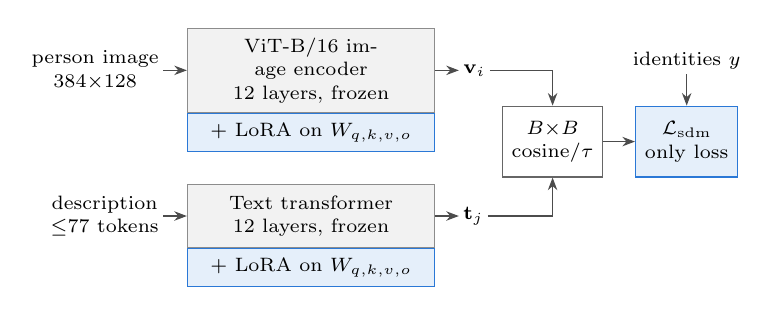
\begin{tikzpicture}[
  font=\fontsize{7}{8.5}\selectfont,
  enc/.style={draw=black!45, fill=black!5, text width=29mm, align=center,
              inner sep=1.2mm, minimum height=8mm},
  lora/.style={draw=cOurs, fill=cOurs!12, text width=29mm, align=center,
               inner sep=1.2mm, minimum height=4.5mm},
  op/.style={draw=black!60, fill=white, align=center, inner sep=1.2mm, minimum height=9mm},
  loss/.style={draw=cOurs, fill=cOurs!12, align=center, inner sep=1.2mm, minimum height=9mm},
  io/.style={align=center, inner sep=0.5mm},
  arr/.style={-{Stealth[length=1.6mm]}, draw=black!70}]
% ---- image lane (top) and text lane (bottom), same x positions
\node[enc]  (vit) at (0, 7.5mm)  {ViT-B/16 image encoder\\12 layers, frozen};
\node[lora, below=0pt of vit]     (lv)  {+ LoRA on $W_{q,k,v,o}$};
\node[enc]  (tr)  at (0,-11mm)   {Text transformer\\12 layers, frozen};
\node[lora, below=0pt of tr]      (lt)  {+ LoRA on $W_{q,k,v,o}$};
\node[io, left=3mm of vit] (img) {person image\\$384{\times}128$};
\node[io, left=3mm of tr]  (txt) {description\\$\le$77 tokens};
\node[io, right=3mm of vit] (v) {$\mathbf{v}_i$};
\node[io, right=3mm of tr]  (t) {$\mathbf{t}_j$};
% ---- similarity and loss, centred between the two lanes
\path (v) -- (t) coordinate[pos=0.5] (mid);
\node[op]   (S) at ($(mid)+(10mm,0)$) {$B{\times}B$\\cosine$/\tau$};
\node[loss, right=4mm of S] (L) {$\mathcal{L}_{\mathrm{sdm}}$\\only loss};
\node[io, above=4mm of L] (y) {identities $y$};
% ---- arrows (orthogonal only)
\draw[arr] (img) -- (vit);
\draw[arr] (txt) -- (tr);
\draw[arr] (vit) -- (v);
\draw[arr] (tr)  -- (t);
\draw[arr] (v) -| (S.north);
\draw[arr] (t) -| (S.south);
\draw[arr] (S) -- (L);
\draw[arr] (y) -- (L);
\end{tikzpicture}

\caption{The pipeline. Grey: frozen CLIP ViT-B/16 (\nBackboneM\,M parameters). Blue: the only trainable parameters, \nLoraModules{} LoRA modules of rank 4 (\nTrainable{} parameters), trained with SDM alone.}
\label{fig:pipeline}
\end{figure}

\subsection{LoRA-tuned CLIP}\label{sec:lora}

Every linear projection inside multi-head attention, the query, key, value and output maps $W\in\mathbb{R}^{d\times d}$, is replaced by
\begin{equation}
W'\mathbf{x}=W\mathbf{x}+\frac{\alpha}{r}\,BA\,\mathbf{x},\qquad A\in\mathbb{R}^{r\times d},\;B\in\mathbb{R}^{d\times r},\label{eq:lora}
\end{equation}
with $W$ frozen, $r=4$ and $\alpha=8$. $A$ is initialised Kaiming-uniform and $B$ to zero, so training starts exactly from pre-trained CLIP. Applying this to both encoders gives $12\times4\times2=\nLoraModules$ modules (\cref{fig:pipeline}). Each module holds $r(d+d)$ parameters, so the image encoder ($d=768$) contributes $48\cdot4\cdot1536=294{,}912$ and the text encoder ($d=512$) $48\cdot4\cdot1024=196{,}608$, a total of \nTrainable, or \trainPct\% of the \nTotalM\,M parameters of the adapted model. Everything else stays frozen, including the embeddings, layer norms, feed-forward blocks, projection heads and the temperature. Since $BA$ can be added to $W$ once training ends, inference costs exactly as much as CLIP's.

\textbf{Objective.} We train with $\mathcal{L}_{\mathrm{sdm}}$ of \cref{eq:sdm} and nothing else. Besides isolating the loss, this keeps the trainable part small: IRRA's ID classifier alone would add $512\times3701$ weights plus biases, \idHeadM\,M parameters or nearly four times our LoRA budget, and the IRR encoder another 13.66\,M. SDM has no parameters and needs the labels only through the relation $y_i=y_j$.

\subsection{What SDM computes with identity labels}\label{sec:analysis}

\textbf{How often does a batch contain a second positive?} SDM differs from InfoNCE only in rows of $q$ that have more than one non-zero entry. RSTPReid's training split contains \nExamples{} image--caption examples, ten per identity (five images, two captions each). With uniform random batches of $B=\batchSize$, as in IRRA's default and our implementation, the probability that a given row has at least one other example of its identity in the batch is
\begin{equation}
1-\prod_{k=0}^{B-2}\frac{N-10-k}{N-1-k}=\posFrac\%,\qquad N=37{,}010.\label{eq:posfrac}
\end{equation}
In \oneHotFrac\% of rows, therefore, $q_{i,\cdot}$ is the one-hot vector $\mathbf{e}_i$, exactly InfoNCE's target. Any difference between SDM and InfoNCE in this regime must come from the form of the loss, not from the targets.

\textbf{SDM with a one-hot target is not InfoNCE.} Substituting $q_{i,\cdot}=\mathbf{e}_i$ into one row of \cref{eq:sdm} and writing $\lambda=\log(1/\epsilon)$ gives
\begin{align}
\ell^{\mathrm{sdm}}_i&=\sum_{j}p_{i,j}\log p_{i,j}+\lambda\sum_{j\neq i}p_{i,j}-p_{i,i}\log(1+\epsilon)\nonumber\\
&\approx \underbrace{\lambda\,(1-p_{i,i})}_{\text{scaled MAE}}\;-\;\underbrace{H(p_{i,\cdot})}_{\text{entropy bonus}},\label{eq:decomp}
\end{align}
with $\lambda=\logInvEps$, whereas InfoNCE's row loss is $\ell^{\mathrm{nce}}_i=-\log p_{i,i}$. The first term is the mean absolute error between $p_{i,\cdot}$ and $\mathbf{e}_i$, $\tfrac12\lVert p_{i,\cdot}-\mathbf{e}_i\rVert_1=1-p_{i,i}$, scaled by $\lambda$; MAE is known to be robust to label noise because it is a symmetric, bounded loss~\cite{ghosh2017robustlossfunctionslabel}. The second term rewards high-entropy predictions, which is the confidence penalty of Pereyra~\textit{et al.}~\cite{pereyra2017regularizingneuralnetworkspenalizing} with weight $1/\lambda\approx0.05$ relative to the first. The two losses share a minimiser, $p_{i,\cdot}=\mathbf{e}_i$, but weight the examples very differently.

\textbf{Gradients.} For logits $z_{i,j}=\mathbf{v}_i^{\top}\mathbf{t}_j/\tau$ and $\tilde q=q+\epsilon$, the exact gradient of one SDM row is
\begin{equation}
\frac{\partial\ell^{\mathrm{sdm}}_i}{\partial z_{i,j}}=p_{i,j}\big(\log p_{i,j}-\log\tilde q_{i,j}-\ell^{\mathrm{sdm}}_i\big),\label{eq:grad}
\end{equation}
while InfoNCE gives $p_{i,j}-\mathbf{1}[j=i]$. On the matching pair, InfoNCE pushes with strength $1-p_{i,i}$, which is largest for the pairs the model ranks worst, while the dominant MAE term of \cref{eq:decomp} pushes with $\lambda\,p_{i,i}(1-p_{i,i})$, which vanishes as $p_{i,i}\to0$. SDM thus concentrates on pairs the model already half-recognises and largely ignores pairs it cannot match, the opposite of InfoNCE's emphasis on the hardest pairs. In TBPS such pairs are often ambiguous rather than informative: two people in near-identical clothing, or a caption that omits the only distinguishing detail.

\textbf{A control loss that isolates the KL direction.} To test whether this, rather than the identity-aware target, explains SDM's advantage, we introduce multi-positive cross-entropy,
\begin{align}
\mathcal{L}^{\mathrm{i2t}}_{\mathrm{mpce}}&=-\frac1B\sum_{i}\sum_{j}q_{i,j}\log p_{i,j}\nonumber\\
&=\frac1B\sum_i\Big[\KL(q_{i,\cdot}\Vert p_{i,\cdot})+H(q_{i,\cdot})\Big],\label{eq:mpce}
\end{align}
summed over both directions as for SDM. MPCE uses exactly SDM's targets but the \emph{forward} KL, and $H(q)$ does not depend on the model. The three losses then form two controlled contrasts: MPCE versus InfoNCE changes only the target (identity-aware or diagonal), and SDM versus MPCE changes only the KL direction. In the one-hot regime MPCE coincides with InfoNCE up to the factor $2$ of \cref{eq:nce}, and Adam-type optimisers are invariant to a constant rescaling of the loss (up to their $\epsilon$ and gradient clipping). Our hypothesis therefore predicts that MPCE will \emph{behave like InfoNCE}, not like SDM. All three identities (\cref{eq:decomp}, MPCE $=2\times$InfoNCE for distinct identities, and SDM $\neq$ InfoNCE) are checked numerically by unit tests in our code.

\section{Experiments \tagO}\label{sec:experiments}

\subsection{Setup}\label{sec:setup}

\textbf{Data and metrics.} RSTPReid~\cite{Zhu_2021} contains 20,505 images of 4,101 identities with two descriptions per image, split into 3,701 training, 200 validation and 200 test identities. The test protocol ranks a gallery of 1,000 images against 2,000 textual queries. We report Rank-$K$ accuracy (R@$K$, the fraction of queries whose first correct image appears in the top $K$), mean average precision (mAP) and mean inverse negative penalty (mINP)~\cite{jiang2023crossmodalimplicitrelationreasoning}. With 2,000 queries, R@1 is a binomial estimate whose standard error is about 1.1 points near 58\%; mAP averages over complete rankings and is less noisy.

\textbf{Training details.} We start from the publicly released CLIP ViT-B/16 weights~\cite{radford2021learningtransferablevisualmodels}. Training images are flipped, padded, randomly cropped and randomly erased, and captions are truncated to 77 tokens. We train with AdamW~\cite{loshchilov2019decoupledweightdecayregularization} (peak learning rate $10^{-4}$, weight decay 0.02), batch size \batchSize, gradient clipping at norm 5 and mixed precision. The learning rate rises linearly over 3 warm-up epochs and then follows a cosine decay to 1\% of its peak; one epoch takes about \sdmMinPerEp{} minutes on a single GPU. The SDM run uses a \sdmRounds-epoch schedule and the InfoNCE and MPCE runs a \nceRounds-epoch schedule, InfoNCE being stopped after \nceEpochs{} epochs. Warm-up is identical, and up to epoch 9 the learning rates stay close (at epoch 4, $\sdmLrFour$ vs.\ $\nceLrFour\times10^{-5}$; at epoch 9, $\sdmLrNine$ vs.\ $\nceLrNine\times10^{-5}$).

\textbf{Protocol.} We evaluate after every epoch. Like IRRA, we report the epoch with the best R@1 (\emph{peak}). Selecting an epoch on the test split is optimistic, so we also report the \emph{converged} value, the mean $\pm$ standard deviation over the last six epochs.

\begin{table*}[t]
\centering
\caption{Results on RSTPReid (text-to-image, \%). Rows marked IRRA are quoted from~\cite{jiang2023crossmodalimplicitrelationreasoning} (Tables 3 and 4 there; that ablation reports no mAP or mINP). Our rows are single runs at their peak epoch; converged values are in \cref{tab:ablation}. ``Stored'' is the size of the trained parameters in fp32.}
\label{tab:main}
\footnotesize
\setlength{\tabcolsep}{3.6pt}
\begin{tabular}{@{}llllrr ccccc@{}}
\toprule
& Method & Tuning & Loss & Trainable & Stored & R@1 & R@5 & R@10 & mAP & mINP\\
\midrule
\multirow{3}{*}{\rotatebox{90}{\scriptsize IRRA}}
& CLIP baseline & full & InfoNCE & 149.6\,M$^\ast$ & \fullMiB\,MiB & 54.05 & 80.70 & 88.00 & 43.41 & 22.31\\
& SDM only (Tab.~4, No.~2) & full & SDM & 149.6\,M$^\ast$ & \fullMiB\,MiB & 57.20 & 79.90 & 88.10 & -- & --\\
& IRRA (full model) & full & SDM+ID+IRR & $>$165\,M$^\dagger$ & $>$630\,MiB & \textbf{60.20} & \textbf{81.30} & 88.20 & \textbf{47.17} & \textbf{25.28}\\
\midrule
\multirow{3}{*}{\rotatebox{90}{\scriptsize Ours}}
& LoRA $r{=}4$ (ep.~\ncePeakEp) & LoRA & InfoNCE & 0.49\,M & \ckptMiB\,MiB & \ncePeakR & \ncePeakRfive & \ncePeakRten & \ncePeakM & \ncePeakMINP\\
& LoRA $r{=}4$ (ep.~\mpcePeakEp) & LoRA & MPCE & 0.49\,M & \ckptMiB\,MiB & \mpcePeakR & \mpcePeakRfive & \mpcePeakRten & \mpcePeakM & \mpcePeakMINP\\
& LoRA $r{=}4$ (ep.~\sdmPeakEp) & LoRA & SDM & 0.49\,M & \ckptMiB\,MiB & \sdmPeakR & \sdmPeakRfive & \textbf{\sdmPeakRten} & \sdmPeakM & \sdmPeakMINP\\
\bottomrule
\end{tabular}\\[2pt]
\parbox{\textwidth}{\scriptsize $^\ast$CLIP ViT-B/16 with position embeddings resampled to the $24{\times}8$ grid (\nBackbone{} parameters). $^\dagger$CLIP plus the 13.66\,M IRR encoder~\cite{jiang2023crossmodalimplicitrelationreasoning} and the \idHeadM\,M ID classifier; the MLM head is not counted.}
\end{table*}

\subsection{LoRA versus full fine-tuning (Q1)}\label{sec:main}

\Cref{tab:main} answers Q1. The fair comparison is IRRA's ablation row that, like ours, uses SDM alone. Full fine-tuning reaches 57.20\% R@1; LoRA reaches \sdmPeakR\% at its peak and \sdmConvR{}$\pm$\sdmConvRsd\% after convergence. The peak is \gapIrraSdmR{} points higher, about 1.5 standard errors, and the converged value matches, so with a single seed we read the two as on par rather than claim an improvement. LoRA gets there with \trainPct\% of the parameters and \ckptMiB\,MiB of trained weights instead of \fullMiB\,MiB. The complete IRRA model, which adds the ID loss and the IRR encoder, is ahead by \gapIrraR{} points of R@1 and \gapIrraM{} of mAP at the peak. Closing that gap would take extra objectives with their own parameters, the trade-off made by the PETL methods in \cref{sec:related}.

\subsection{Where does SDM's gain come from? (Q2)}\label{sec:ablation}

\begin{table}[t]
\centering
\caption{Loss ablation with LoRA $r{=}4$ (single seed, \%). Only the loss differs. Converged values average the last six epochs of each run's own schedule.}
\label{tab:ablation}
\footnotesize
\setlength{\tabcolsep}{3pt}
\begin{tabular}{@{}lllccc@{}}
\toprule
Loss & Target & Divergence & Peak R@1 (ep.) & Peak mAP & Conv.\ R@1\\
\midrule
InfoNCE & diagonal & CE & \ncePeakR{} (\ncePeakEp) & \ncePeakM & \nceConvR{}$\pm$\nceConvRsd\\
MPCE & identity & $\KL(q\Vert p)$ & \mpcePeakR{} (\mpcePeakEp) & \mpcePeakM & \mpceConvR{}$\pm$\mpceConvRsd\\
SDM & identity & $\KL(p\Vert q)$ & \textbf{\sdmPeakR} (\sdmPeakEp) & \textbf{\sdmPeakM} & \textbf{\sdmConvR}$\pm$\sdmConvRsd\\
\bottomrule
\end{tabular}
\end{table}

\begin{figure}[t]
\centering
\begin{tikzpicture}
\pgfplotsset{
  every axis/.append style={width=\columnwidth,height=3.55cm,xmin=0.5,xmax=30.5,
    tick label style={font=\scriptsize},label style={font=\scriptsize},
    grid=major,grid style={black!12},axis line style={black!45},tick style={black!45}},
  sdm/.style={cSDM,thick,mark=*,mark size=1.3pt},
  mpce/.style={cMPCE,thick,dashed,mark=triangle*,mark size=1.6pt,mark options={solid}},
  nce/.style={cNCE,thick,densely dotted,mark=square*,mark size=1.1pt,mark options={solid}}}
\begin{axis}[name=top,ylabel={R@1 (\%)},ymin=40,ymax=61,xticklabels={}]
\addplot[sdm] table[x=epoch,y=r1,col sep=comma]{generated/curve_sdm.csv};
\addplot[mpce] table[x=epoch,y=r1,col sep=comma]{generated/curve_mpce.csv};
\addplot[nce] table[x=epoch,y=r1,col sep=comma]{generated/curve_nce.csv};
\draw[cIRRA,thin,dashdotted] (axis cs:0.5,57.20) -- (axis cs:30.5,57.20) node[pos=0.98,above left,font=\tiny,inner sep=1pt]{IRRA full FT, SDM 57.20};
\draw[cIRRA,thin,dashdotted] (axis cs:0.5,54.05) -- (axis cs:30.5,54.05) node[pos=0.98,above left,font=\tiny,inner sep=1pt]{IRRA full FT, InfoNCE 54.05};
\end{axis}
\begin{axis}[at={(top.south)},anchor=north,yshift=-1.5mm,xlabel={epoch},ylabel={mAP (\%)},ymin=30,ymax=47,
  legend style={font=\scriptsize,at={(0.99,0.04)},anchor=south east,draw=black!30,fill=white,legend columns=3}]
\addplot[sdm] table[x=epoch,y=map,col sep=comma]{generated/curve_sdm.csv};
\addplot[mpce] table[x=epoch,y=map,col sep=comma]{generated/curve_mpce.csv};
\addplot[nce] table[x=epoch,y=map,col sep=comma]{generated/curve_nce.csv};
\legend{SDM,MPCE,InfoNCE}
\end{axis}
\end{tikzpicture}
\caption{Test R@1 and mAP after each epoch. MPCE and InfoNCE peak at the end of warm-up and then decline together; SDM keeps improving. Grey lines: IRRA's full fine-tuning results~\cite{jiang2023crossmodalimplicitrelationreasoning}.}
\label{fig:curves}
\end{figure}

\Cref{tab:ablation} and \cref{fig:curves} compare the three losses under identical LoRA training. SDM leads InfoNCE by \gapSdmNceR{} points of R@1 and \gapSdmNceM{} of mAP at the peak, close to the \gainIrraSdm{} points IRRA reports for full fine-tuning, so LoRA keeps SDM's benefit. The ablation also shows where that benefit comes from.

\textbf{Identity-aware targets contribute nothing measurable.} MPCE and InfoNCE share the same \nPairedEp-epoch schedule, so they can be compared epoch by epoch. Across these epochs MPCE's R@1 differs from InfoNCE's by \mpNceDiffR{}$\pm$\mpNceDiffRsd{} points on average (largest gap \mpNceDiffRmax) and its mAP by \mpNceDiffM{} (largest \mpNceDiffMmax), both well inside run-to-run noise. The ratio of their training losses stays between \lossRatioLo{} and \lossRatioHi, as \cref{sec:analysis} predicts: exactly 2 for one-hot rows, slightly more because of the \posFrac\% of rows with an extra positive, which confirms that the targets are almost always one-hot.

\textbf{The KL direction accounts for the whole gain.} SDM and MPCE share the target and differ only in the direction of the divergence, and SDM leads MPCE by \gapSdmMpceR{} points of R@1 and \gapSdmMpceM{} of mAP at the peak. The curves show how this gap arises. InfoNCE and MPCE peak at epoch 3, the end of warm-up, and then lose \nceDrop{} and \mpceDrop{} points of R@1 while their training losses keep falling (InfoNCE from \nceLossFirst{} to \nceLossLast), the usual sign of overfitting. SDM instead climbs until epoch \sdmPeakEp{} and ends within \sdmDrop{} points of its peak. Over epochs 4--9 the learning rates of the two schedules differ by at most \lrMaxRelDiff\%, yet the curves move in opposite directions (SDM from \sdmEpFourR{} to \sdmEpNineR, InfoNCE from \nceEpFourR{} to \nceEpNineR), so the schedule difference cannot explain the gap.

\textbf{Interpretation.} Under random sampling, IRRA's rationale for SDM, that it accounts for several positives per batch, applies to fewer than 2\% of rows and cannot explain a three-point gain. \Cref{eq:decomp,eq:grad} offer an explanation consistent with the curves: InfoNCE spends the largest gradients on the pairs it ranks worst, which on a small dataset with ambiguous descriptions leads it to memorise them, whereas SDM's bounded, MAE-like term down-weights those pairs and its entropy bonus discourages over-confident similarity distributions. We have not separated the two terms experimentally, so this remains a hypothesis, but the decomposition makes it testable: varying $\epsilon$ rescales $\lambda$ and with it the weight of the MAE term against the entropy bonus, and each term can be trained alone.

\subsection{Implications for federated training}\label{sec:fl}

\begin{table}[t]
\centering
\caption{What the trainable-part size implies for a federation of $K{=}\kClients$ clients (one per RSTPReid camera) over $R{=}\rRounds$ rounds. Arithmetic from the parameter counts (fp32), not a measurement; downloads from the server double the traffic.}
\label{tab:cost}
\footnotesize
\setlength{\tabcolsep}{4pt}
\begin{tabular}{@{}lrrr@{}}
\toprule
 & Full FT & LoRA $r{=}4$ & Ratio\\
\midrule
Trainable parameters & \nBackboneM\,M & 0.49\,M & \sizeRatio$\times$\\
Upload per client per round & \fullMiB\,MiB & \ckptMiB\,MiB & \sizeRatio$\times$\\
Upload per round ($K$ clients) & \upFullRoundGiB\,GiB & \upLoraRoundMiB\,MiB & \sizeRatio$\times$\\
Upload over $R$ rounds & \upFullTotalGiB\,GiB & \upLoraTotalGiB\,GiB & \sizeRatio$\times$\\
AdamW state per client & \optFullGiB\,GiB & \optLoraMiB\,MiB & \sizeRatio$\times$\\
\midrule
R@1, SDM only (peak / conv.) & 57.20 / -- & \sdmPeakR{} / \sdmConvR & \\
\bottomrule
\end{tabular}
\end{table}

\Cref{tab:cost} turns the parameter count into the quantities that dominate FL, assuming that every client takes part in every round and uploads its whole trainable part. With full fine-tuning each round would send \upFullRoundGiB\,GiB upstream, a heavy load for camera-side clients, whereas a whole LoRA round sends \roundVsOneFull$\times$ less than a single client's full-model upload. Each client's optimiser state shrinks by the same factor, which matters on edge hardware. Together with \cref{sec:main}, this is the premise a federated PEFT design for TBPS needs: the \sizeRatio$\times$ reduction costs no measurable accuracy against SDM-only full fine-tuning and \gapIrraR{} points of R@1 against the complete IRRA model.

The loss analysis carries over too. Unlike IRRA's ID classifier, whose rows refer to identities that other clients may never see, SDM has no parameters tied to the global identity set, so it can be optimised locally and averaged without modification. And since SDM's gain does not depend on several images of one person sharing a batch (\cref{sec:ablation}), there is no reason to expect it to vanish on clients with few images per identity. Whether these arguments hold under non-IID clients and the averaging of low-rank factors can only be settled by a federated experiment, which is beyond this report.

\section{Limitations}\label{sec:limits}

Every run uses one seed, and R@1 on RSTPReid carries a standard error of about 1.1 points, so differences below roughly two points (LoRA versus full fine-tuning with SDM) should be read as parity; the SDM-versus-InfoNCE and SDM-versus-MPCE gaps are about three standard errors and are mirrored in the less noisy mAP. The SDM run used a shorter learning-rate schedule than the other two; \cref{sec:ablation} argues that this does not explain the result, but a matched rerun would remove the caveat. All conclusions concern RSTPReid with random batch sampling. On larger datasets, or with an identity-balanced sampler that places several images of each person in a batch, the multi-positive targets of SDM and MPCE become frequent and may then matter. The IRRA numbers are quoted from the paper rather than reproduced, and the mechanism proposed in \cref{sec:ablation} has not yet been isolated experimentally. Finally, no federated experiment is reported: \cref{sec:fl} is an accounting argument, and how accuracy behaves under non-IID clients remains to be measured in the thesis.

\section{Conclusion}\label{sec:conclusion}

This report tested, in the centralised setting, the premise behind using PEFT for federated text-based person search: that a far smaller trainable part loses little accuracy. Starting from IRRA, we asked how much accuracy a frozen CLIP backbone retains with LoRA and the SDM loss alone, and why SDM helps. With \trainPct\% of the parameters, \sizeRatio$\times$ fewer than full fine-tuning, LoRA+SDM matches IRRA's fully fine-tuned SDM-only model on RSTPReid (\sdmPeakR\% peak, \sdmConvR\% converged, against 57.20\%) and trails the complete IRRA model by \gapIrraR{} points of R@1, while cutting the per-round upload of a \kClients-client federation from \upFullRoundGiB\,GiB to \upLoraRoundMiB\,MiB. The premise holds. On the second question our evidence contradicts the usual explanation. Under random sampling SDM's targets are one-hot in \oneHotFrac\% of rows; in that regime SDM is a scaled mean-absolute-error loss plus an entropy bonus rather than InfoNCE, and a control loss with SDM's targets but the forward KL behaves exactly like InfoNCE. The benefit of SDM therefore lies in the direction of its divergence, which resists the overfitting that InfoNCE shows on this small dataset. Next steps are seeded reruns with a common schedule, ablations of the two terms of \cref{eq:decomp}, an identity-balanced sampler, and, in the thesis, federated training of LoRA+SDM over camera-level clients on RSTPReid, CUHK-PEDES and ICFG-PEDES.


\bibliographystyle{IEEEtran}
\bibliography{refs}

\end{document}
